% Schematic curves from E:/网页下载/fig_response_threshold_band.tex.
\documentclass[tikz,border=2pt]{standalone}
% Shared typography and colors for the manuscript's standalone TikZ figures.
\usepackage[T1]{fontenc}
\usepackage{lmodern}
\usepackage{amsmath,amssymb,bm}
% Keep the text design used by the 10.95 pt manuscript body when source
% lettering is enlarged to compensate for includegraphics scaling.
\DeclareFontShape{T1}{lmr}{m}{n}{<->ec-lmr10}{}
\DeclareFontShape{T1}{lmr}{m}{it}{<->ec-lmri10}{}
\DeclareFontShape{T1}{lmr}{bx}{n}{<->ec-lmbx10}{}
\usetikzlibrary{arrows.meta}
\definecolor{ink}{HTML}{253139}
\definecolor{blueink}{HTML}{52758A}
\definecolor{linegray}{HTML}{65747E}
\definecolor{guidegray}{HTML}{AEBBC4}
\definecolor{framegray}{HTML}{C9D2D8}
\definecolor{safefill}{HTML}{D5E6F1}
\definecolor{overlapfill}{HTML}{F7E6AF}
\definecolor{failurefill}{HTML}{EFC6C1}
\definecolor{intervalink}{HTML}{9B752B}

% At 0.50*495 pt inclusion width, this gives approximately 10.95 pt in print.
\tikzset{
  font=\fontsize{17.33}{20.80}\selectfont,text=ink,
  labelsmall/.style={font=\fontsize{17.33}{20.80}\selectfont},
  axisarrow/.style={-{Stealth[length=5pt,width=5pt]},line width=1.1pt,draw=ink},
  bound/.style={draw=blueink,line width=1.4pt},
  truecdf/.style={draw=ink,line width=1.1pt,dash pattern=on 4pt off 3pt},
  guide/.style={draw=guidegray,line width=.55pt,densely dashed},
  leader/.style={draw=linegray,line width=.65pt,-{Stealth[length=4pt,width=4pt]}},
  interval/.style={draw=intervalink,line width=1.8pt}
}
\newcommand{\bandkey}{\tikz[baseline=4pt]{%
  \draw[fill=safefill,draw=blueink,line width=.8pt] (0,0) rectangle (13pt,13pt);}}
\newcommand{\cdfkey}{\tikz[baseline=-.45ex]{%
  \draw[truecdf] (0,0)--(17pt,0);}}
\newcommand{\intervalkey}{\tikz[baseline=4pt]{%
  \draw[interval] (0,0)--(0,13pt);
  \foreach \y in {0,13pt}
    \node[circle,draw=intervalink,fill=overlapfill,inner sep=0pt,minimum size=5pt,line width=.8pt] at (0,\y) {};}}

\begin{document}
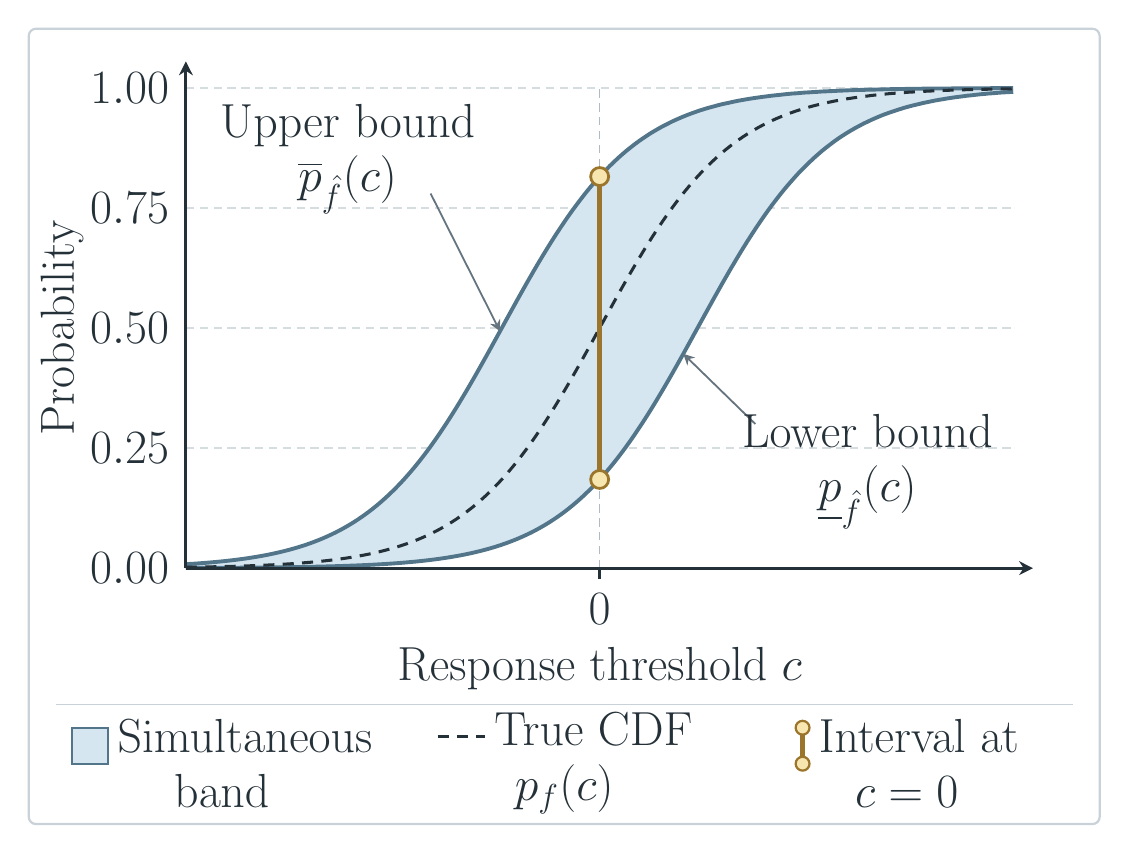
\begin{tikzpicture}[x=1cm,y=1cm]
  \draw[draw=framegray,line width=.8pt,rounded corners=2.6pt]
    (0,0) rectangle (13.6,10.1);
  % The supplied logistic functions and their horizontal shifts are preserved.
  \pgfmathdeclarefunction{uppercdf}{1}{\pgfmathparse{1/(1+exp(-1.35*(#1+1.1)))}}
  \pgfmathdeclarefunction{lowercdf}{1}{\pgfmathparse{1/(1+exp(-1.35*(#1-1.1)))}}
  \pgfmathdeclarefunction{truecdf}{1}{\pgfmathparse{1/(1+exp(-1.35*#1))}}
  \pgfmathsetmacro{\plo}{lowercdf(0)}
  \pgfmathsetmacro{\phi}{uppercdf(0)}
  \begin{scope}[shift={(7.25,3.25)},x=1.13cm,y=6.10cm]
    \foreach \p/\lab in {0/0.00,.25/0.25,.5/0.50,.75/0.75,1/1.00}{
      \draw[draw=guidegray!50,line width=.55pt,densely dashed] (-4.65,\p)--(4.65,\p);
      \node[anchor=east,labelsmall,inner sep=3pt] at (-4.74,\p) {$\lab$};
    }
    \fill[safefill]
      plot[domain=-4.65:4.65,samples=200] (\x,{uppercdf(\x)})
      -- plot[domain=4.65:-4.65,samples=200] (\x,{lowercdf(\x)}) -- cycle;
    \draw[guide] (0,0)--(0,1);
    \draw[bound] plot[domain=-4.65:4.65,samples=200] (\x,{uppercdf(\x)});
    \draw[bound] plot[domain=-4.65:4.65,samples=200] (\x,{lowercdf(\x)});
    \draw[truecdf] plot[domain=-4.65:4.65,samples=200] (\x,{truecdf(\x)});
    \draw[interval] (0,\plo)--(0,\phi);
    \foreach \p in {\plo,\phi}
      \node[circle,draw=intervalink,fill=overlapfill,inner sep=0pt,
        minimum size=6.5pt,line width=1pt] at (0,\p) {};
    \draw[axisarrow] (-4.65,0)--(4.87,0);
    \draw[axisarrow] (-4.65,0)--(-4.65,1.055);
    \draw[ink,line width=.85pt] (0,0)--(0,-.022);
    \node[anchor=north,labelsmall,inner sep=3pt] at (0,-.035) {$0$};
    \draw[leader] (-1.90,.78)--(-1.12,{uppercdf(-1.12)});
    \draw[leader] (1.75,.30)--(.94,{lowercdf(.94)});
  \end{scope}
  \node[align=center,inner sep=0pt] at (4.05,8.45)
    {Upper bound\\[-1pt]$\overline p_{\hat f}(c)$};
  \node[align=center,inner sep=0pt] at (10.65,4.48)
    {Lower bound\\[-1pt]$\underline p_{\hat f}(c)$};
  \node[rotate=90] at (.42,6.30) {Probability};
  \node at (7.25,1.98) {Response threshold $c$};
  \draw[draw=framegray,line width=.55pt] (.34,1.52)--(13.26,1.52);
  % Three centered columns keep full-size legend text inside the user's width.
  \node[align=center,inner sep=0pt] at (2.45,.77)
    {\bandkey\hspace{3pt}Simultaneous\\[-1pt]band};
  \node[align=center,inner sep=0pt] at (6.80,.77)
    {\cdfkey\hspace{3pt}True CDF\\[-1pt]$p_f(c)$};
  \node[align=center,inner sep=0pt] at (11.15,.77)
    {\intervalkey\hspace{3pt}Interval at\\[-1pt]$c=0$};
\end{tikzpicture}
\end{document}
